Il sistema corrente presenta una \textit{three-tier architecture} in cui sono presenti i classici 3 layer: \textit{presentation}, \textit{application} e \textit{storage}. 

\begin{figure}[h!]
	\centering
	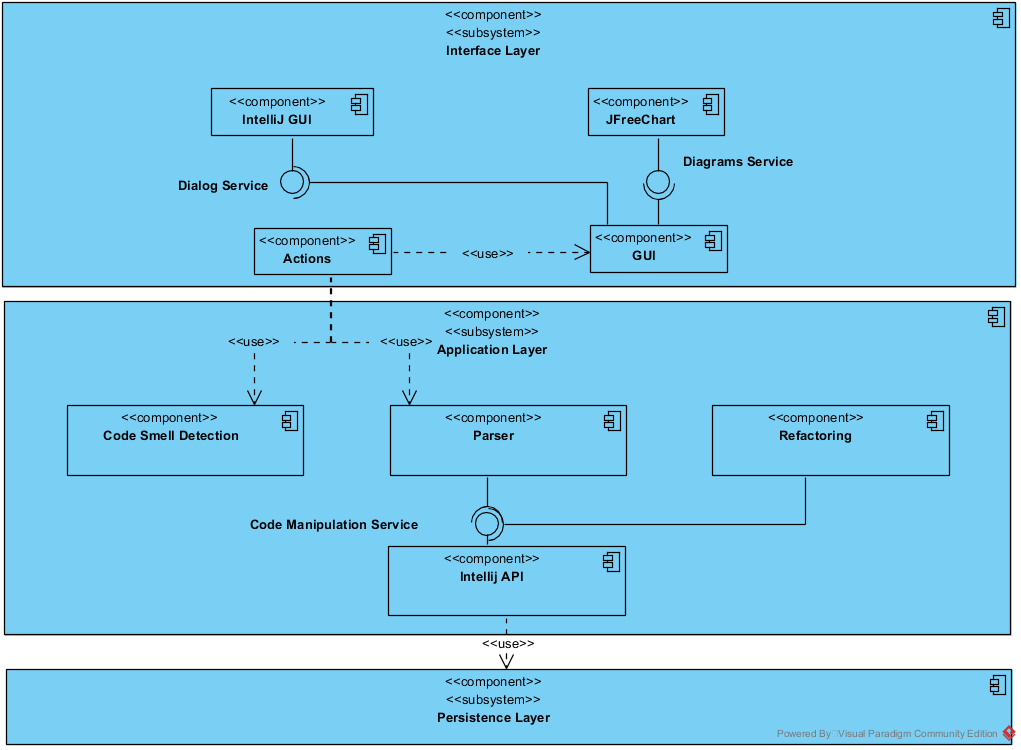
\includegraphics[scale=0.7]{./CS_Architecture/Diagrams/TACOR-Component.png} \\
	\textbf{Current Architecture Overview}
\end{figure}


\paragraph{}Il \textit{presentation layer} include tutte le interfacce grafiche e le \textit{actions}, ovvero componenti che, opportunamente configurate, eseguono codice in risposta a interazioni dell'utente con componenti grafiche estese dell'IDE. Queste componenti fungono, dunque, da connettori tra Intellij e il codice del plugin.

\paragraph{} L' \textit{application layer} contiene tutto il codice di business del plugin ed è composto da 3 componenti principali: \textit{Code Smell Detection}, \textit{Parser} e \textit{Refactoring}. Il primo si occupa delll'individuazione dei code smell all'interno dei componenti codice sotto analisi, il secondo di ricavare dal codice in esame le informazioni necessarie al \textit{Code Smell Detection} per effettuare le analisi, mentre il terzo si occupa di mettere in atto le operazioni di refactoring correttive dei \textit{code smell}. Tutti e tre sono utilizzati e coordinati dalle classi \textit{actions} e dagli \textit{action listeners} delle interfacce grafiche e quindi utilizzati come se fossero un \textit{Service Layer} che agisce su classi che mantengono solamente dati, i beans. Tutto ciò indica che il plugin presenta un'architettura, come la definisce Martin Fowler, \textit{anemica}.

\paragraph{} Lo \textit{storage layer}, invece, è costituito dai files contenente il codice sorgente in esame. Esso non viene mai acceduto direttamente dal codice di business del plugin, ma attraverso le API offerte dalla piattaforma Intellij.

\paragraph{} Le modifiche presenti nella sezione 3 consistono in una rimodulazione e ristrutturazione generale dell'architettura, volte a risolvere i problemi di manutenibilità e la mancata adesione all'object-orientation che derivano dall'architettura anemica del sistema. Inoltre, tale ristrutturazione rende più semplice l'aggiunta delle due nuove funzionalità di correzione di \textit{Blob} e \textit{Promiscuous Package}. Per ulteriori dettagli, si fa riferimento al documento di \textit{Change Impact Analysis}.  